\graphicspath{{Ch2_background/}}

\chapter{Background\label{sec:bg}}

We consider prediction problems where we are given inputs and need to make some decision about them. In the context of image recognition, let us consider images of natural objects (\eg dogs) as input. The task is to predict semantic content in the image. We will consider the image classification task where a single label per image (\eg `dog' or `person') must be predicted, and more complex tasks where rich description (\eg `dog on surfboard') must be predicted (\fig{\ref{fig:problem}}).%\looseness-1

\begin{figure}[htbp]
    \centering
     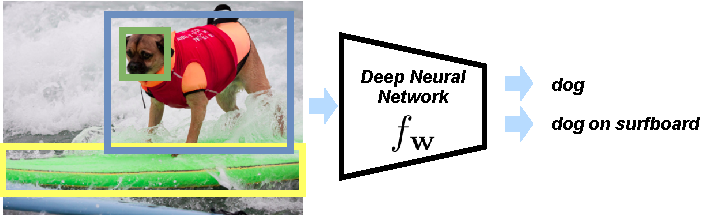
\includegraphics[width=0.9\textwidth, align=c]{figs/problem_form.pdf} 
    \caption{Prediction of object categories and their relationships given an image.}
    \label{fig:problem}
\end{figure}


\section{Neural networks\label{sec:bg_nn}}
In image recognition tasks,
%, such as image classification, 
the input is high dimensional\footnote{Image resolution varies drastically between image tasks, but generally represent high-dimensional cases. For example, in MNIST~\citep{lecun1998gradient}, the images are 28$\times$28 pixels, \ie 784 dimensional. In more realistic tasks, such as PASCAL~\citep{everingham2010pascal}, images can be 500$\times$300 pixels, \ie 150,000 dimensional.} and the decision process is hard to formally describe using simple expert rules and raw inputs.
Therefore, the currently dominant strategy to solve such a task is to formulate it as an optimization problem:
%
\begin{equation}
    \w^* = \underset{\w}{\text{arg\,min }} \ \mathcal{L}(f_\w, \mathcal{D}),
\end{equation} 
%
%$\in \mathcal{D}$
\noindent where $f_\w$ is some function parameterized by $\w$, $\mathcal{D}$ is the dataset associated with the task and $\mathcal{L}$ is the objective to minimize for this dataset. The goal of solving this problem is to find optimal parameters $\w^*$ for $f_\w$.
For large and complex datasets, the state-of-the-art solutions to this optimization problem are often based on using deep neural networks (DNNs) as $f_\w$. Finding globally optimal $\w^*$ of DNNs is generally intractable due to the highly non-convex nature of $\mathcal{L}(f_\w, \mathcal{D})$~\citep{choromanska2015loss}. Nevertheless, local optima can be found using methods based on gradient descent~\citep{ruder2016overview,kingma2014adam}.\looseness-1

%The design of DNNs varies drastically depending on the task. 
DNNs can have drastically different designs depending on the task. This thesis concerns three different designs of DNNs. The first is one of the earliest types of DNNs, colloquially referred to as a multilayer perceptron (MLP). Next, we consider convolutional neural networks (\cnns) -- DNNs designed specifically for perceptual tasks, such as image recognition. Lastly, we consider graph neural networks (\gnns) that are designed for graph-structured data. MLPs, \cnns and \gnns are the core building blocks of this thesis.
%\footnote{Some portions of \S~\ref{sec:bg_nn} are based on my blog posts: \url{https://medium.com/@BorisAKnyazev}}.

\subsection{Multilayer perceptrons\label{sec:bg_mlp}}
MLPs or, more precisely, multilayer feedforward fully-connected neural networks, consist of $L$ layers of trainable parameters (weights) $\w = [\W^{(1)}, \W^{(2)}, ..., \W^{(L)}]$. Given $N$ input data points $\X \in \R^{N \times d} $ of dimensionality $d$ from the dataset $\mathcal{D}$, the MLP sequentially transforms the input $\X$ as\footnote{For simplicity, in \eqref{eq:mlp} we ignore the bias term $\mathbf{b}$ that in practice is added to the output of $\X^{(l)}\W^{(l)}$. The bias is essential when a single layer is used, however it has limited practical value in the case of $L > 1$.}:
%
\begin{equation}
    \label{eq:mlp}
    \X^{(l+1)} = \sigma(\X^{(l)}\W^{(l)}),
\end{equation}
%
\noindent where $l \in [1,L]$ and an input to the first layer $\X^{(1)}$ is equal to $\X$. Function $\sigma$ is some nonlinearity such as the Rectified Linear Unit (ReLU) applied element-wise to $\X^{(l)}\W^{(l)}$: $\sigma (\X^{(l)}\W^{(l)})=\max(0, \X^{(l)}\W^{(l)})$. More advanced nonlinearities can lead to better training and generalization properties, e.g. leaky ReLU~\citep{maas2013rectifier} or the Exponential Linear Unit (ELU)~\citep{clevert2015fast}. Applying $\sigma$ is essential to learn nonlinear transformations. One of the simplest nonlinear transformations is the XOR logic operation that was famous in diminishing the interest in AI (``AI winter'') in the 1970s\footnote{More about that period can be read at \url{https://dev.to/jbahire/demystifying-the-xor-problem-1blk} or \url{https://towardsdatascience.com/history-of-the-first-ai-winter-6f8c2186f80b}.}. For the final layer ($l=L$), it is common to use a nonlinearity specific for the task. For example, in the case of predicting binary labels $\mathbf{y} \in [0,1]^N$ for data points $\X$, a sigmoid function can be applied. In the case of regression tasks, $\mathbf{y} \in \R^N$, \ie, the final nonlinearity is removed.
All $N$ data points in $\X$ can be processed by MLPs independently, so parallel computing enables very efficient usage of MLPs. $N$ data points processed in parallel are often called a mini-batch, or batch\footnote{When ``batch'' and ``mini-batch'' are used to describe the operation of learning, batch means updates based on the entire dataset and mini-batch means updates based on a subset.}.\looseness-1
%Multiple layers with interleaved nonlinearities are required to learn such and more complex transformations.
%For example an MLP with a single layer of parameters $\W \in \R^{d_1 \times d_2}$: $f(\X, \W) = \X\W$. 
%The MLP layers can be stacked to form a deep network: $f(\X, \W) = (\sigma(\X\W^{1}))\W^{2}$, where $\sigma$ is some nonlinearity such as ReLU to learn a nonlinear transformations. 
%Without $\sigma$ multiple layers will be equivalent to a single layer thus preventing learning complex transformations.
\paragraph{Applications of MLPs.} MLPs can be in principle applied to any tabular data $\X$ where rows are data points and columns are features or dimensions. While images can be represented as tabular data by flattening spatial dimensions~\citep{ciregan2012multi}, MLPs are more common in cases when the dimensions in $\X$ are not ordered in any meaningful way (\ie there is no benefit of leveraging the order).
%(\ie the order can be changed without affecting the training procedure).
MLPs are often used as building blocks of many other types of DNNs, including recently developed Transformers~\citep{vaswani2017attention,dosovitskiy2020image} and Graph Neural Networks~\citep{kipf2016semi} (\S~\ref{sec:bg_gnn}). Oftentimes, the last few layers of Convolutional Neural Networks (\S~\ref{sec:bg_cnn}) are modeled as MLPs~\citep{simonyan2014very}.
Recently, models based on MLPs were revisited in large-scale image tasks, where they showed competitive results~\citep{touvron2021resmlp}.\looseness-1

\subsection{Convolutional neural networks\label{sec:bg_cnn}}

The main building blocks of \cnns, convolution and downsampling, were introduced in~\citep{fukushima1982neocognitron}.
%Convolution and downsampling are the main building blocks of CNNs~\citep{fukushima1982neocognitron}. 
Subsequently, in \citep{lecun1998gradient}, \cnns were combined with a gradient descent-based training algorithm to effectively learn the parameters of \cnns from raw inputs (images) without manually engineering features.
Following~\eqref{eq:mlp} for the MLP layer, the convolutional layer for $N$ images ${\cal X} \in \R^{N \times C \times H \times W}$ and $K$ filters (kernels, weights) $\mathcal{W} \in \R^{K \times C \times h \times w}$ can be defined as~\citep{vedaldi2015matconvnet}:
%
\begin{equation}
    \label{eq:conv}
    {\cal X}_{n,k,i,j}^{(l+1)} = \sigma(\sum_c \sum_h \sum_w {\cal X}_{n,c,i-h,j-w}^{(l)} {\cal W}_{k,c,h,w}^{(l)}),
\end{equation}
%
\noindent where $C$ is the number of channels (\eg $C=3$ for RGB images); $H,W$ are the height and width of images respectively; $K$ is the number of filters and $h,w$ are their height and width respectively. Each $k$-th filter of $\mathcal{W}$ slides over the input along the spatial dimensions and for each spatial location $i \in [1,H], j \in [1,W]$ of $\mathcal{X}$ computes the dot product between the local region and the kernel (\fig{\ref{fig:conv}}).\looseness-1


\begin{figure}[htbp]
    \centering
    \footnotesize
    \begin{tabular}{cccc}
    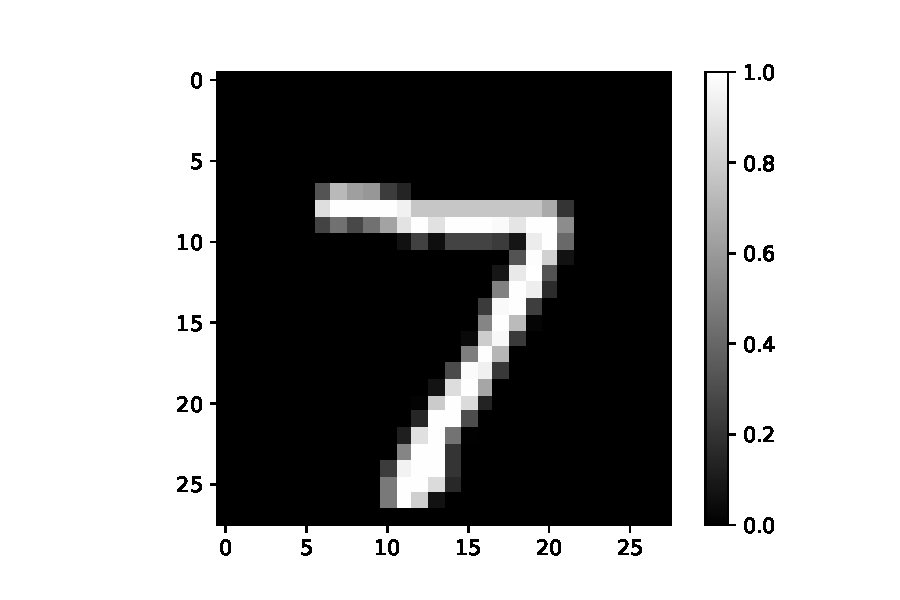
\includegraphics[width=0.22\textwidth]{figs/mnist_digit.pdf} & 
    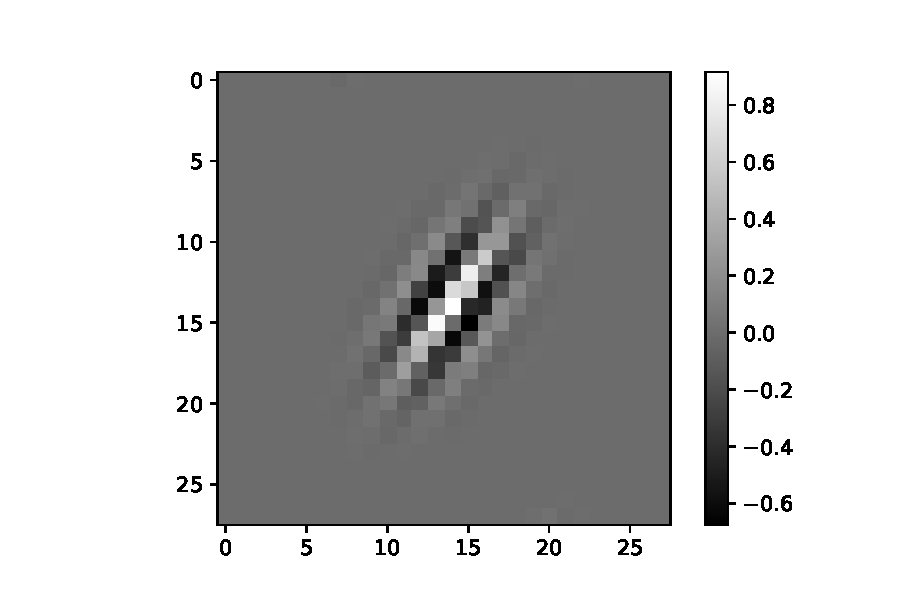
\includegraphics[width=0.22\textwidth]{figs/conv_kernel.pdf} & 
    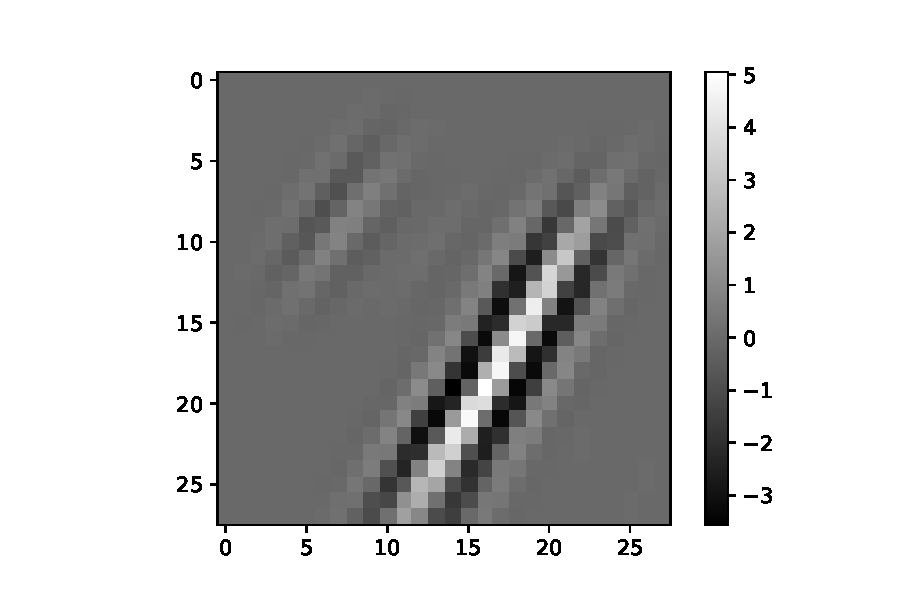
\includegraphics[width=0.22\textwidth]{figs/conv_output.pdf} & 
    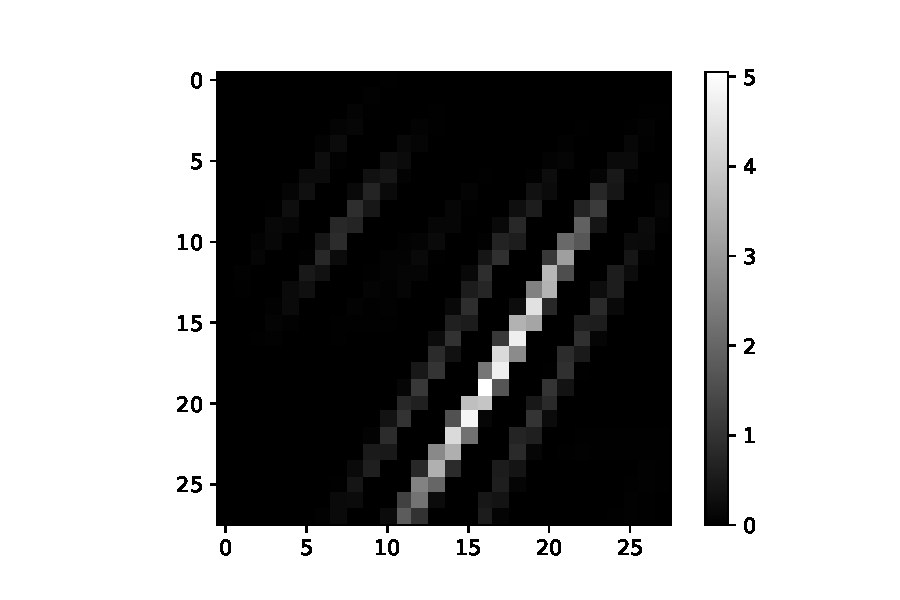
\includegraphics[width=0.22\textwidth]{figs/relu_output.pdf} \\
    Input image & Convolutional filter & Output of convolution & Output after ReLU \\
    \end{tabular}
    \caption{Example of the convolution operation for a single image and single filter.}
    \label{fig:conv}
\end{figure}

The convolution operation exploits a 2D local structure in images, formally described in~\citep{bronstein2017geometric}:
\vspace{-3pt}
\begin{itemize}
    \setlength{\itemsep}{1pt}
    \item Shift-invariance -- if we spatially translate an object on the image to the left/right/up/down, we still should be able to recognize it. This is exploited by sharing filters across all locations.
    \item Locality -- nearby pixels are closely related and often represent some semantic concepts, such as object parts. This is exploited by using filters with spatial dimensions $h > 1$ and $w > 1$, which can capture image features in a local spatial neighborhood.
    \item Compositionality (or hierarchy) -- a larger region in the image is often a semantic parent of smaller regions it contains. For example, a dog is a parent of a head, body, legs, etc. 
    %Likewise, the head is a parent of ears, nose, eyes, etc. 
    This implicitly is exploited by stacking convolutional layers.
\end{itemize}

Another important component of \cnns is the downsampling operation. Downsampling reduces the spatial size of inputs, which is important for computational efficiency, particularly for large inputs. Downsampling is usually based on spatial pooling applied to a local region similar to convolution. Typically, average or max poolings are used that do not have trainable parameters. In practice, pooling can be replaced with modified (strided) convolution to simplify the overall network~\citep{springenberg2014striving}.\looseness-1

As compared to MLPs, \cnns applied to images have another strength besides those listed above. In particular, the number of trainable parameters in convolutional filters $\mathcal{W}$ does not depend on the input spatial dimensions $H,W$. In principle, the same \cnn can be trained on images with $H=W=28$ as well as $H=W=500$. In addition, \cnns are highly efficient due to their ability to apply filters $\mathcal{W}$ independently and in parallel for each spatial location, each filter and each image. As a result, \cnns have been adapted to a broad range of tasks beyond image classification.
%In other words, the model is parametric.

\vspace{-3pt}
\paragraph{Applications of \cnns.} \cnns initially were proposed for simple image classification tasks, such as handwritten digit recognition (MNIST)~\citep{lecun1998gradient}. Subsequently, a larger and deeper network proposed in \citep{krizhevsky2012imagenet} led to the top-1 result on the ImageNet 2012 challenge of large-scale image classification~\citep{russakovsky2015imagenet} outperforming hand-designed visual features such as SIFT~\citep{lowe2004distinctive}.
Compared to~\citep{lecun1998gradient}, the main changes made in \citep{krizhevsky2012imagenet} to \cnns were: i) dramatically increased size of a \cnn possible due to larger and cheaper computational resources available, ii) a large annotated dataset (\ie ImageNet), iii) applying nonlinearities and regularization methods such as ReLU and Dropout~\citep{hinton2012improving}.
Since then, \cnns have dominated visual tasks~\citep{gu2018recent} and grown significantly in size showing superior results in image and video object
%(\eg a dog, a surfboard in \fig{\ref{fig:problem}})
detection~\citep{ren2015faster,wang2017video,he2016deep,he2015delving}, image and video semantic segmentation~\citep{long2015fully,shelhamer2016clockwork}, video recognition~\citep{simonyan2014two}, image and video generation~\citep{goodfellow2014generative,vondrick2016generating}, learning to estimate the optical flow between a pair of images~\citep{dosovitskiy2015flownet}, and many other tasks.
In these and more complex tasks, such as visual question answering (VQA)~\citep{antol2015vqa}, \cnns are typically used as a ``backbone'' to extract visual features from images. The same backbone and its trained parameters can be used across different tasks. The procedure of reusing the backbone parameters from one task to improve on another task is called ``transfer learning''. Typically, backbones trained on large image tasks such as ImageNet show the best transfer learning abilities~\citep{huh2016makes,kornblith2019better}.
%``Transfer learning'' is a common practice in/for X that transfer \cnns pretrained on large image datasets such as ImageNet. 
Finally, \cnns' computational efficiency has been significantly improved. In particular, architectural enhancements~\citep{howard2017mobilenets,cai2019onceforall}, as well as compression and distillation techniques~\citep{cheng2017survey} together with very efficient implementations~\citep{chetlur2014cudnn} enabled the deployment of \cnns on low-resource mobile devices further extending \cnns' application reach.\looseness-1
% to a downstream task
%For example, object detectors predict a set of bounding boxes (x,y,width,height) for each object and their category. In \fig{\ref{fig:problem}} the object detector should detect a dog, surfboard, wave and, ideally, fine-grained details such as vest and dog's body parts.
%The widespread utility of \cnns is reinforced by their efficiency, which is due to the parallelization of the convolution operation. \looseness-1

%\cnns are the main backbone of computer vision models, such as object detectors~\citep{ren2015faster}. 

\subsection{Graph neural networks\label{sec:bg_gnn}}

The wide success of \cnns have motivated their application to more tasks.
%methods in other tasks where 
%One of such tasks is learning from graph-structured data. 
In tasks such as chemistry, physics and social networks,
% Graph-structured data are ubiquitous in
%, transportation, 3D geometry, visual reasoning, and others
the data are represented as graphs. 
%However, applying \cnns to graphs is not straightforward as there is no notion of spatial translation in graphs. 
However, convolution \eqref{eq:conv} requires data to reside on a ``regular grid'', a Euclidean coordinate system where all the data points are located at the discrete and equally spaced coordinates consistent among all samples~\citep{bronstein2017geometric}. For example, all MNIST images reside on the same 28$\times$28 regular grid. In contrast, graphs generally reside on ``irregular grids'' that do not have a notion of spatial translation, preventing the application of convolution as per \eqref{eq:conv}.\looseness-1

Formally, a graph $\G$ consists of an unordered set of $N$ nodes, $\V$, connected by edges, $\E$. 
The edges are often encoded by an adjacency matrix $\A \in \R^{N \times N}$. The number of neighbors for each node can be then defined as a diagonal matrix $\D$, where $\D_{ii} = \sum_j \A_{ij}$. %, which is binary if the graph is unweighted.
Defining convolution on graphs is non-trivial because the nodes are generally unordered, and not attached to a particular coordinate system, and the node degree $\D_{ii}$ can vary for each $i$-th node.

To define convolution on graphs, a spectral graph theory has been applied~\citep{bruna2013spectral}. This theory is based on extending the spectral definition of convolution in signal processing. For signals, we can define spectral convolution equivalent to the spatial definition in~\eqref{eq:conv} using the Discrete Fourier Transform. Similarly, spectral convolution on graphs can be computed~\citep{belkin2001laplacian,chung1997spectral,bruna2013spectral}\footnote{An extended description of defining spectral convolution on graphs can be found in my blog post: \url{https://towardsdatascience.com/spectral-graph-convolution-explained-and-implemented-step-by-step-2e495b57f801}.} based on the eigendecomposition of the graph Laplacian $\Lapl = \mathbf{I}_N - \D^{-1/2}\A\D^{-1/2}$, where $\mathbf{I}_N$ is an $N \times N$ identity matrix. In particular, the eigendecomposition of $\Lapl$ is defined as $\Lapl=\mathbf{V}\mathbf{\Lambda}\mathbf{V}^T$, where $\mathbf{V}$ are eigenvectors and $\mathbf{\Lambda}$ are eigenvalues.
Given node features $\X^{(l)} \in \R^{N \times d}$, the spectral graph convolution layer with filters $\W^{(l)}$ can be then defined as:
%
\begin{equation}
 \label{eq:graph_spectral_conv}    
 \X^{(l+1)} = \sigma \Big( \mathbf{V} (\mathbf{V}^T\X^{(l)} \odot \mathbf{V}^T\W^{(l)}) \Big),
\end{equation}
%
\noindent where $\odot$ is element-wise multiplication. Similarly to the spectral convolution in signal processing, in \eqref{eq:graph_spectral_conv} the features and filters are first projected into the spectral domain where they are multiplied. The result is then reconstructed back to the original domain.

A major disadvantage of spectral graph convolution defined in \eqref{eq:graph_spectral_conv} is the necessity to compute the eigendecomposition for each graph. In many graph tasks, graphs have very different structures (and different eigenvectors $\mathbf{V}$) and it is unclear if the same $\W^{(l)}$ can adapt to different $\mathbf{V}$~\citep{nilsson2020experimental}. 
%For example, at test time, for a new graph and a new set of eigenvectors, these filters might be inappropriate.
Moreover, computing eigendecomposition for large graphs is a computationally intensive process.
To eliminate the need of eigendecomposition, %\citet{defferrard2016convolutional} proposed to approximate \eqref{eq:graph_spectral_conv} with Chebyshev polynomials of order $K \in [1, N]$. Chebyshev convolution aggregates node features within the $K$-hop neighborhood. 
spectral graph convolution \eqref{eq:graph_spectral_conv} can be approximated using recursive Chebyshev polynomials $T_k$ and the property of eigendecomposition that $\Lapl^k=(\mathbf{V} \mathbf{\Lambda} \mathbf{V}^T)^k = \mathbf{V} \mathbf{\Lambda}^k \mathbf{V}^T$.
To derive approximate Chebyshev graph convolution, 
the polynomials $T_k$ are first applied to the rescaled graph Laplacian $\tilde{\Lapl}=2\Lapl/\lambda_{\max} - \mathbf{I}_N$~\citep{hammond2011wavelets, defferrard2016convolutional}:\looseness-1
%
\begin{equation}
\label{eq:cheb_lapl}
T_k(\tilde{\Lapl}) = 2 \tilde{\Lapl} T_{k-1}(\tilde{\Lapl}) - T_{k-2}(\tilde{\Lapl}), 
\end{equation}
%
\noindent where $k \in [1, N]$, $T_0(\tilde{\Lapl}) = \mathbf{I}_N$ and $T_1(\tilde{\Lapl}) = \tilde{\Lapl}$; $\lambda_{\max}$ is the largest eigenvalue of $\Lapl$.
Using \eqref{eq:cheb_lapl} and the aforementioned property of eigendecomposition that $\Lapl^k= \mathbf{V} \mathbf{\Lambda}^k \mathbf{V}^T$, \citet{hammond2011wavelets, defferrard2016convolutional} derived that spectral graph convolution can be approximated as a sum of the $T_k(\tilde{\Lapl})$ terms weighted by trainable parameters $\W^{(l)}_k$. Hence, the Chebyshev graph convolution layer can be defined as:
%
\begin{equation}
\label{eq:cheb_graph_conv}
\X^{(l+1)} = \sigma \Big(\sum^{K-1}_{k=0} T_k(\tilde{\Lapl}) \X^{(l)} \W^{(l)}_k \Big),
\end{equation}
%
\noindent where $K \in [1, N]$ is a hyperparameter controlling how global is the receptive field of the convolution. In particular, the terms $T_k(\tilde{\Lapl})$ include powers $\tilde{\Lapl}^k$ enabling a $(k-1)$-hop receptive field and allowing to approximate spectral convolution. For example, for $K=N$ the convolution \eqref{eq:cheb_graph_conv} is performed globally based on the entire graph structure making it approximately equal to spectral convolution \eqref{eq:graph_spectral_conv}. For $K=1$ we have $T_0(\tilde{\Lapl}) = \mathbf{I}_N$, so the convolution is performed ignoring the graph structure, while for $K=2$ the convolution is performed based on the 1-hop neighborhood of nodes, and so forth.
Stacking Chebyshev graph convolution layers \eqref{eq:cheb_graph_conv} form a graph neural network called a ChebyNet studied in our works~\citep{knyazev2018spectral,knyazev2019image,knyazev2019understanding}.

\citet{kipf2016semi} studied the 1-hop Chebyshev graph convolution (with $K=2$) and proposed its highly-effective and efficient simplification:\looseness-1
%
\begin{equation}
    \label{eq:graph_conv_kipf}
    \X^{(l+1)} = \sigma(\hat{\A}\X^{(l)}\W^{(l)}),
\end{equation}
%
\noindent where $\hat{\A}$ is a normalized adjacency matrix similar to the rescaled graph Laplacian $\tilde{\Lapl}$: $\hat{\A} = \tilde{\D}^{-1/2}\tilde{\A}\tilde{\D}^{-1/2}$, and $\tilde{\D}_{ii} = \sum_j \tilde{\A}_{ij}$; $\tilde{\A} = \A + I_N$ to include self-loops into convolution. Essentially, \eqref{eq:graph_conv_kipf} combines the first two terms of \eqref{eq:cheb_graph_conv} for $k=[1,2]$ into a single operation. The model based on multiple convolutions \eqref{eq:graph_conv_kipf} is commonly referred to as a graph convolutional network (GCN). In this thesis, we will use a more general term ``graph neural network'' (\gnn) to refer to this and other graph models.\looseness-1

The graph layer defined in~\eqref{eq:graph_conv_kipf} is remarkably similar to the one of the MLP layer~\eqref{eq:mlp}. The only difference is the normalized adjacency matrix $\hat{A}$ used in~\eqref{eq:graph_conv_kipf}. Therefore, a \gnn can be viewed as an MLP exploiting the relational information between data points (or node features). 

Following the example in \fig{\ref{fig:conv}} (\S~\ref{sec:bg_cnn}), graph convolution \eqref{eq:graph_conv_kipf} can be illustrated based on an MNIST image. To represent an image as a graph, nodes correspond to pixel coordinates and edges connect only four spatially adjacent pixels (\fig{\ref{fig:graph_conv}}). In the graphs, pixel intensities are inverted for better visualization with black nodes corresponding to white pixels. The image is resized to 14$\times$14 and a small amount of Gaussian noise is added to illustrate the effect of graph convolution. To compute the output, only $\hat{\A}\X^{(l)}$ is used while $\W^{(l)}$ is ignored. Such graph convolution is equivalent to a low-pass mean filter commonly used in signal processing to denoise the signal. The low-pass effect helps \gnns to excel in tasks where aggregating 1-hop node features is sufficient for high performance. However, 1-hop low-pass filtering also limits the expressive power of \gnns in tasks where complex long-range interactions between nodes are important~\citep{nt2019revisiting,knyazev2019image}.~\looseness-1


\begin{figure}[htbp]
    \centering
    \newcommand{\figwidth}{0.16\textwidth}
    \begin{tabular}{ccc}
        {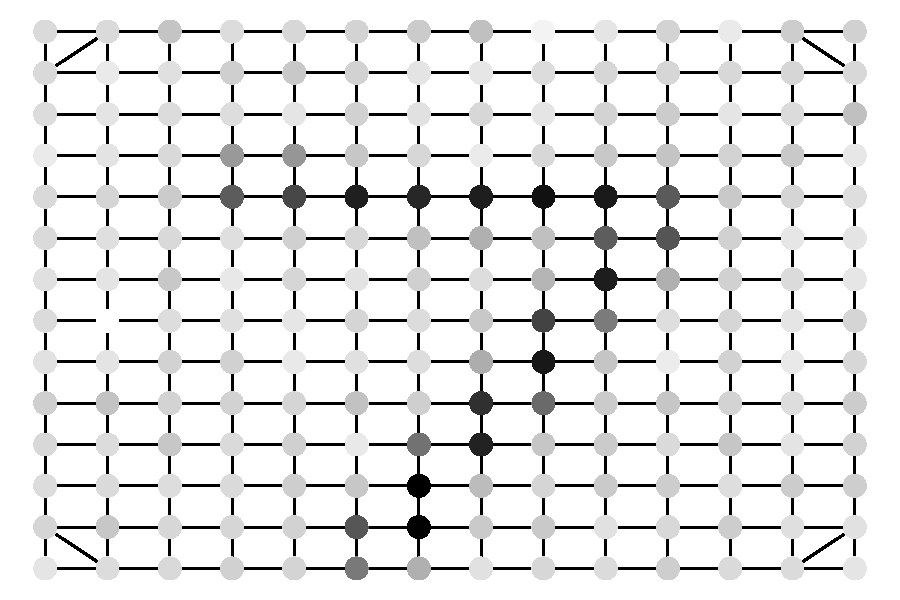
\includegraphics[width=\figwidth,height=\figwidth,clip,trim={1.65cm 0 1.65cm 0}]{figs/graph_conv_in.pdf}} &  
        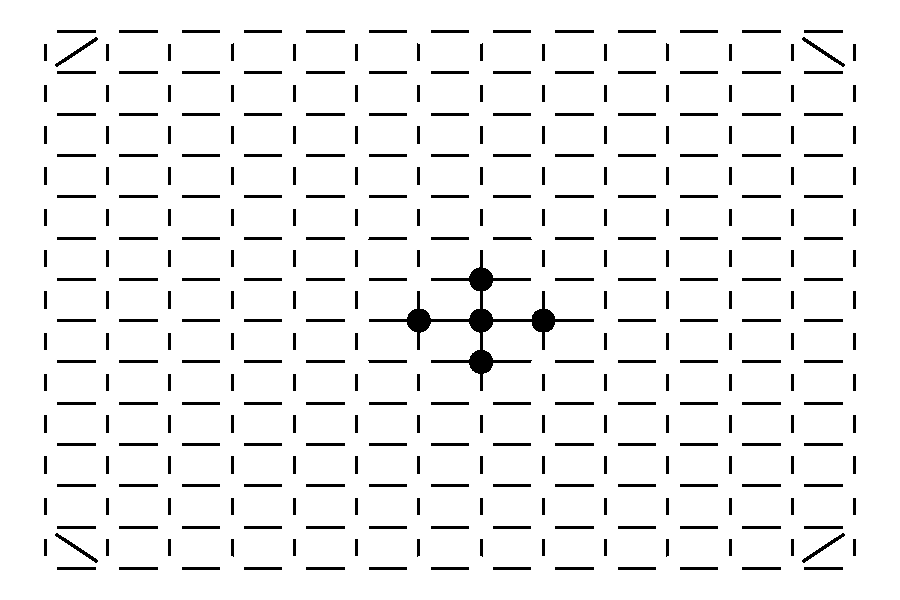
\includegraphics[width=\figwidth,height=\figwidth,clip,trim={1.65cm 0 1.65cm 0}]{figs/graph_conv_kernel.pdf} &
        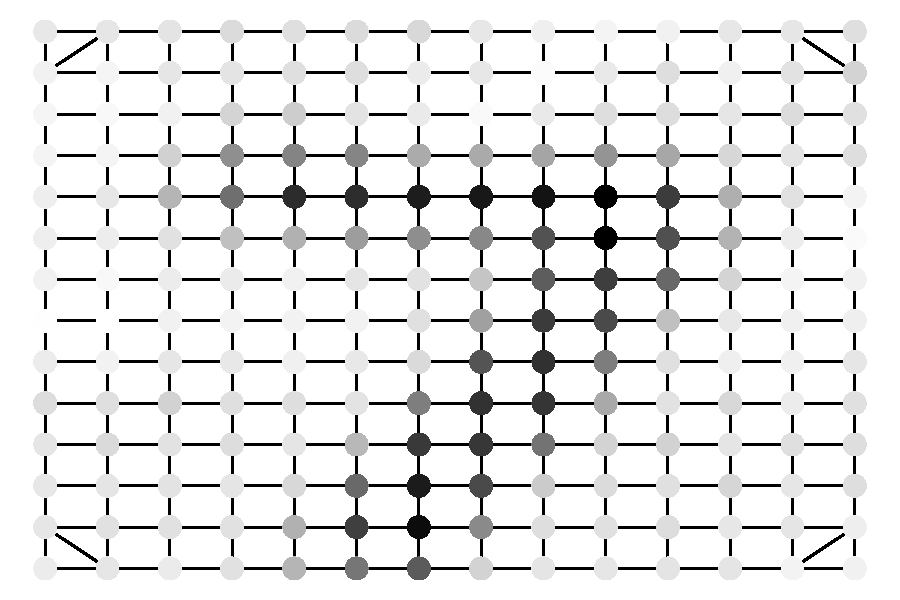
\includegraphics[width=\figwidth,height=\figwidth,clip,trim={1.65cm 0 1.65cm 0}]{figs/graph_conv_out.pdf} \\
        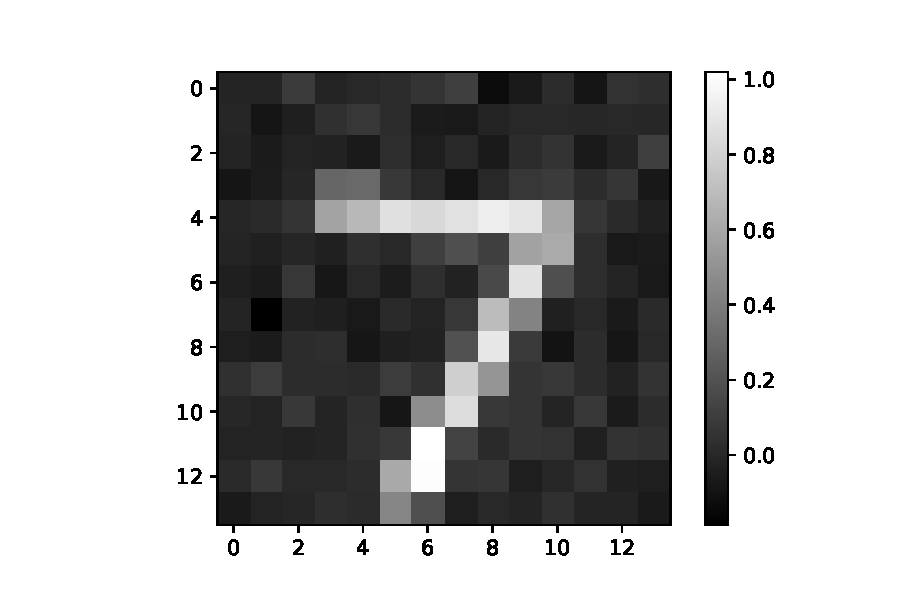
\includegraphics[width=0.27\textwidth]{figs/graph_conv_in_im.pdf} &  
        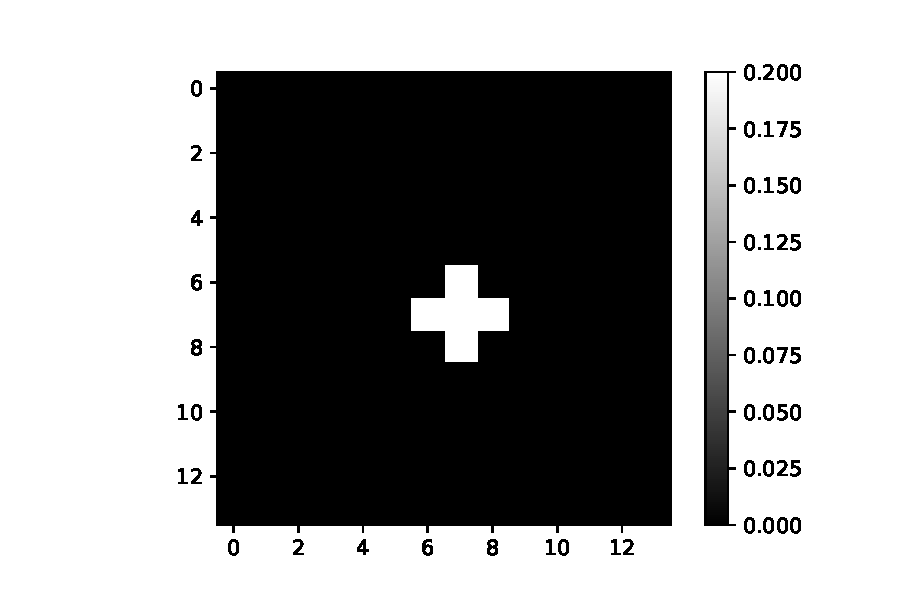
\includegraphics[width=0.27\textwidth]{figs/graph_conv_kernel_im.pdf}
        &
        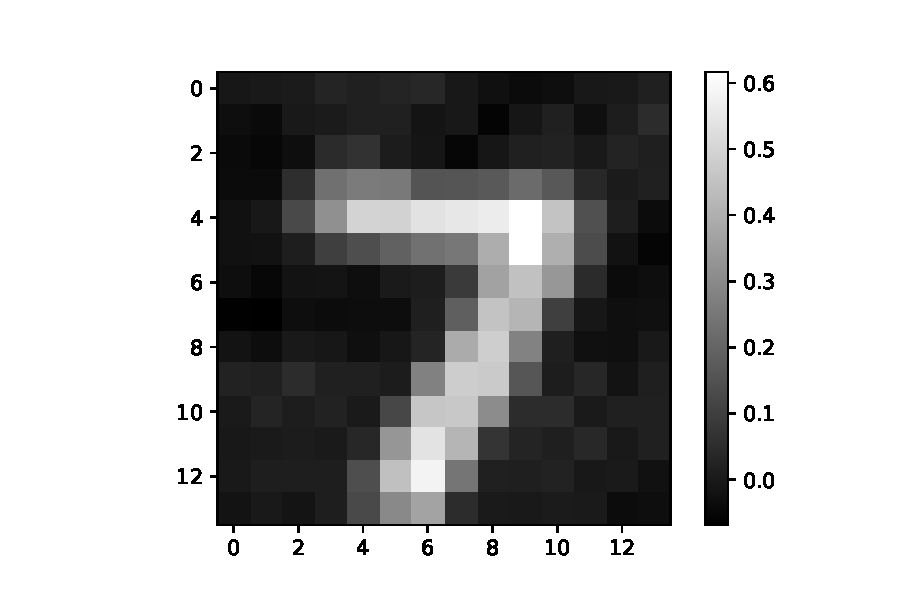
\includegraphics[width=0.27\textwidth]{figs/graph_conv_out_im.pdf} \\
        Input graph/image & Convolutional filter & Output graph/image \\
    \end{tabular}
    \caption{Example of the graph convolution operation for a single graph and single filter.}
    \label{fig:graph_conv}
\end{figure}


\vspace{-3pt}
\paragraph{Extensions of \gnns.}
\gnns were first proposed as early as in 1997 by~\citet{sperduti1997supervised} and subsequently integrated with recurrent neural networks in~\citep{gori2005new,scarselli2008graph}.
The works of~\citet{defferrard2016convolutional} and~\citet{kipf2016semi} synergized with deep learning and the \gnns field has grown considerably.
Notable extensions include Graph Attention Networks~\citep{velickovic2017graph} that learn pairwise attention between nodes to better capture regularities in graphs. Graph Isomorphism Networks~\citep{xu2018how} and Principal Neighbourhood Aggregation~\citep{corso2020principal} use novel more expressive feature aggregation strategies to better differentiate graphs and showed one of the best results in a large-scale graph benchmark~\citep{hu2020open}. Simple GCNs~\citep{wu2019simplifying} propose a single layer \gnn that is computationally efficient yet performant in many tasks. 
Message Passing Networks~\citep{gilmer2017neural,battaglia2018relational} generalize \gnns to support edge features in addition to node features. 
Gated \gnns~\citep{li2015gated} extended earlier \gnns~\citep{gori2005new,scarselli2008graph} based on recurrent networks and recently showed top results among other \gnns in different tasks~\citep{dwivedi2020benchmarking}.

\vspace{-3pt}
\paragraph{Applications of \gnns.} \gnns primarily focus on solving node and graph classification tasks and link prediction~\citep{hamilton2017representation,wu2020comprehensive,battaglia2018relational}. Graph generation~\citep{you2018graphrnn,liao2019efficient} and analysis of dynamic graphs~\citep{kazemi2019relational,trivedi2019dyrep} are also becoming common tasks. Graphs can be used to model virtually any kind of data, so besides solving classic graph tasks such as molecule classification~\citep{xu2018how,knyazev2018spectral}, \gnns have been recently applied to more diverse tasks: image classification~\citep{knyazev2019image,meyer2020large}, semantic segmentation~\citep{li2018beyond,zhang2019dual}, visual relationship detection~\citep{xu2017scene,yang2018graph}, modelling neural network architectures~\citep{zhang2018graph,wen2020neural}, program synthesis~\citep{zhang2018neural}, learning interactions between elements of complex systems~\citep{kipf2018neural,bapst2019structured} and many other tasks. Such a wide range of tasks shows a great potential of \gnns and, therefore, \gnns are a central focuses of this thesis.\looseness-1

\paragraph{Alternatives to \gnns.} Recently, Transformers~\citep{vaswani2017attention,dosovitskiy2020image} have become competitive in diverse tasks. In principle, these models are capable of capturing graph-structured data if the relational information is properly modelled. For example, if relative positional encoding is used~\citep{shaw2018self}, Transformers can learn a graph representation similar to such \gnns as GATs~\citep{velickovic2017graph}. The relation between Transformers and \gnns has been more formally confirmed in~\citep{dwivedi2020generalization,yun2019graph}.


\paragraph{Graph pooling.} Like \cnns, \gnns can exploit the local structure of data to perform some type of downsampling or pooling of the input graph.
In \gnns, pooling methods generally follow the same idea as in \cnns. However, in \gnns the pooling regions (sets of nodes) are often found based on clustering, since there is no regular grid as in images~\citep{defferrard2016convolutional,shaham2018spectralnet,ying2018hierarchical}.
Differently from clustering-based graph pooling, top-k pooling was proposed~\citep{graphunet2018}. Instead of clustering ``similar'' nodes, top-k propagates only part of the input disregarding the rest.
%Top-k pooling can thus select some part of the input graph disregarding the rest. 
%For this reason at first glance it does not appear to be logical.
Formally, given node features $\X^{(l)}$ for layer $l$, the output node features $\mathbf{Z}^{(l)}$ of top-k pooling can be defined as:\looseness-1
%However, we can notice that pooled feature maps in~\cite[Eq.~2]{graphunet2018} are computed in the same way as attention outputs $\mathbf{Z}$ in Eq.~\ref{eq:attn} above, if we rewrite their Eq.~2 in the following way:
%
\begin{equation}
%\label{eq:top-k}
%	Z_i = \alpha_i X_i, \forall i \in P, Z_i = \emptyset, \forall i \notin P
%\[
\mathbf{Z}^{(l)}_i =
\begin{cases}
\mathbf{a}_i \X^{(l)}_i,& \forall i \in P\\
\emptyset, & \text{otherwise} ,
\end{cases}
%\]
\end{equation}
%
where $P$ is a set of indices of pooled nodes, $|P| \leq N$, and $\emptyset$ denotes the unit is absent in the output. $\mathbf{a} \in \R^N$ is predicted by some auxiliary subnetwork: $\mathbf{a}=f(\X^{(l)}, \A)$, where for $f$ a \gnn can be used as in~\citep{lee2019self} or an MLP ignoring the graph structure (adjacency matrix $\A$) can be used as in~\citep{graphunet2018}.
The indices $P$ are the indices of the $|P|$ largest (top) values in $\mathbf{a}$.

Both \gnns and \cnns are built by stacking convolutional and pooling layers to form a deep network. Sometimes, \cnns are augmented with \gnns to improve learning in visual tasks~\citep{li2018beyond,liu2020non}.\looseness-1

\section{Compositional and graph reasoning\label{sec:bg_comp}}

With the basic building blocks, MLPs, \cnns and \gnns, we can build systems that solve complex \textit{compositional reasoning} tasks. In this thesis, by compositional reasoning we assume the process of making a decision by analyzing the collection, or \textit{composition}, of entities where the entities can refer to graph nodes and edges; objects, object parts and relations; or abstract concepts or patterns (\eg subgraphs, strokes, stripes).
In this section, we will describe compositional reasoning methods that mainly concern vision tasks, since these tasks are well studied and easy to understand with simple examples. But similar tasks and methods solving them exist in different domains of compositional reasoning, such as graph reasoning~\citep{hamilton2018embedding} or natural language processing~\citep{lake2018generalization}.\looseness-1

A classic example of compositional visual reasoning is visual question answering (VQA)~\citep{antol2015vqa}. In VQA, the decision is the answer obtained by visually reasoning over a set of objects and relationships between them given a question, \eg \textit{how many chairs are on the left of the table in this image?}. Simpler tasks such as classifying images can also be considered as visual reasoning tasks. Visual reasoning methods may be grouped into low-level and high-level ones and different methods are used in each case. 
%The methods proposed in \S~\ref{sec:completed} and \S~\ref{sec:proposal} will concern both of these groups and, in fact, will be aimed to bridge the gap between them in the context of a specific problem -- compositional generalization.\looseness-1

\subsection{Low-level compositional reasoning\label{sec:bg_low}}
% Explain image classification as a low-level reasoning
We can view image classification as a low-level visual reasoning task, since the model needs to recognize low-level components and relate them to each other in order to make an accurate prediction.
%the category of the object in an image
The low-level components can be object attributes and parts, parts of parts, or even individual pixels.
%in case of tasks such as MNIST~\citep{lecun1998gradient} . 
Reasoning over object parts and attributes rather than making a direct decision about an image enables more explainable decisions~\citep{ul2019explaining} and zero-shot object classification~\citep{lampert2013attribute,demirel2017attributes2classname,naeem2021learning,tokmakov2019learning}. 
For example, a relatively complex zebra image can be recognized if the model detects stripes, a tail, a head, long legs (\fig{\ref{fig:attrib}}a). A simple MNIST image can be recognized based on the composition of strokes and other patterns (\fig{\ref{fig:attrib}}b).
Regardless of image complexity, the lowest level of reasoning is individual pixels. In complex images, the compositions of individual pixels are less likely to directly lead to a particular semantic decision. However, individual pixels can still affect the prediction of object parts and attributes, which in turn can affect the final prediction. Therefore, it is important to consider low-level reasoning both in simple and complex images to develop more robust and explainable models.\looseness-1
%compared to simple images. 
%So in complex images, low-this form of reasoning is rather abstract. 
%Since this reasoning still affects the final decision, it can be called ``hidden'' reasoning. Low-level reasoning includes all these different forms of reasoning.
%\paragraph{Hidden reasoning}
%By low-level reasoning we will also assume pixel level reasoning that does not directly lead to a particular decision. Maybe call this hidden reasoning?


\begin{figure}[htbp]
    \centering
    \setlength{\tabcolsep}{10pt}
    \begin{tabular}{cc}
         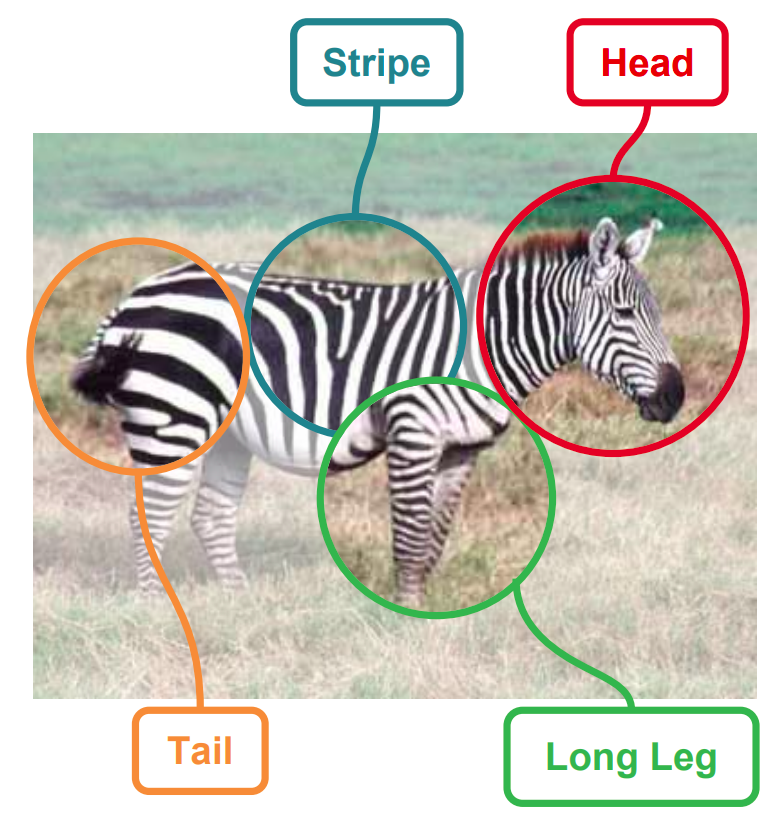
\includegraphics[width=0.3\textwidth,align=c]{figs/zebra_atrib.png}
         & 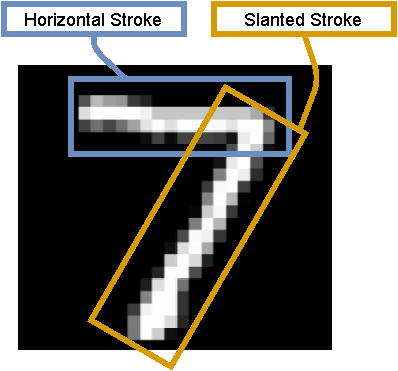
\includegraphics[width=0.3\textwidth,align=c]{figs/mnist_atrib.pdf} \\
         (a) & (b)
    \end{tabular}
    \vspace{-5pt}
    \caption{ (a) A zebra can be described as a collection of object parts, patterns and attributes (figure from~\citep{demirel2017attributes2classname}); (b) A digit can be described as a collection of primitive strokes and patterns.}
    \label{fig:attrib}
    \vspace{-10pt}
\end{figure}

\subsection{High-level compositional reasoning\label{sec:bg_high}}
\vspace{-3pt}

High-level visual reasoning has been more extensively  studied in different tasks than low-level reasoning. The most common, and perhaps, comprehensive high-level reasoning task is Visual Question Answering (VQA)~\citep{antol2015vqa,johnson2017clevr}. One of the ways to effectively solve VQA is to first extract a semantic image description -- a scene graph~\citep{NSM2019,yi2018neural,zhang2019empirical}. 
Formally, a scene graph~\citep{johnson2015image} ${\cal G}=(O,R)$ consists of a set of subjects and objects ($O$) as nodes and a set of relationships or predicates ($R$) between them as edges. The nodes and edges form visual relationship \textit{triplets}: $\langle$\textit{subject}, \textit{predicate}, \textit{object}$\rangle$, \eg
% $\langle$person, on, surfboard$\rangle$, 
$\langle$cup, on, table$\rangle$. %Each node in the graph corresponds to a subject or object (with a specific image location) and edges correspond to predicates. 
%Besides bridging the gap, SGs can be used to verify how well the model has understood the visual world, as opposed to just exploiting one of the biases in a dataset~\citep{jabri2016revisiting,anand2018blindfold,bahdanau2018systematic}.
% Thus, scene graphs are semantic descriptions of images. 
Solving VQA becomes much easier when the input to the question-answering module is semantic, such as a scene graph, rather than raw pixels or abstract features. Similar to VQA, in image captioning~\citep{yang2019auto, gu2019unpaired} and retrieval~\citep{johnson2015image,belilovsky2017joint,tang2020unbiased}, extracting a scene graph from images also simplifies the task improving the downstream performance. Inferring a scene graph is also beneficial for explainable visual reasoning~\citep{shi2019explainable} within the explainable AI (XAI) paradigm~\citep{gunning2019darpa}, since the final predictions can be traced back to semantic concepts of scene graphs.
Extracting a scene graph generally requires a predefined vocabulary of concepts, which is a time-consuming process that must be done for each new task. Therefore, a more flexible strategy is to describe images using abstract entities~\citep{norcliffe2018learning,vedantam2019probabilistic,locatello2020object,burgess2019monet,greff2020binding} that, if necessary, can be tied to semantic concepts (see \S~\ref{sec:bg_methods}).\looseness-1
% -- a semantic collection of objects and relationships between them. 
%As reasoning over abstract entities is not necessary high-level, so the corresponding methods are reviewed separately in § 3.2.4.
% \begin{figure}[thbp]
% 	\centering
% 	\begin{scriptsize}
% 		\setlength{\tabcolsep}{1pt}
% 		\begin{tabular}{c} 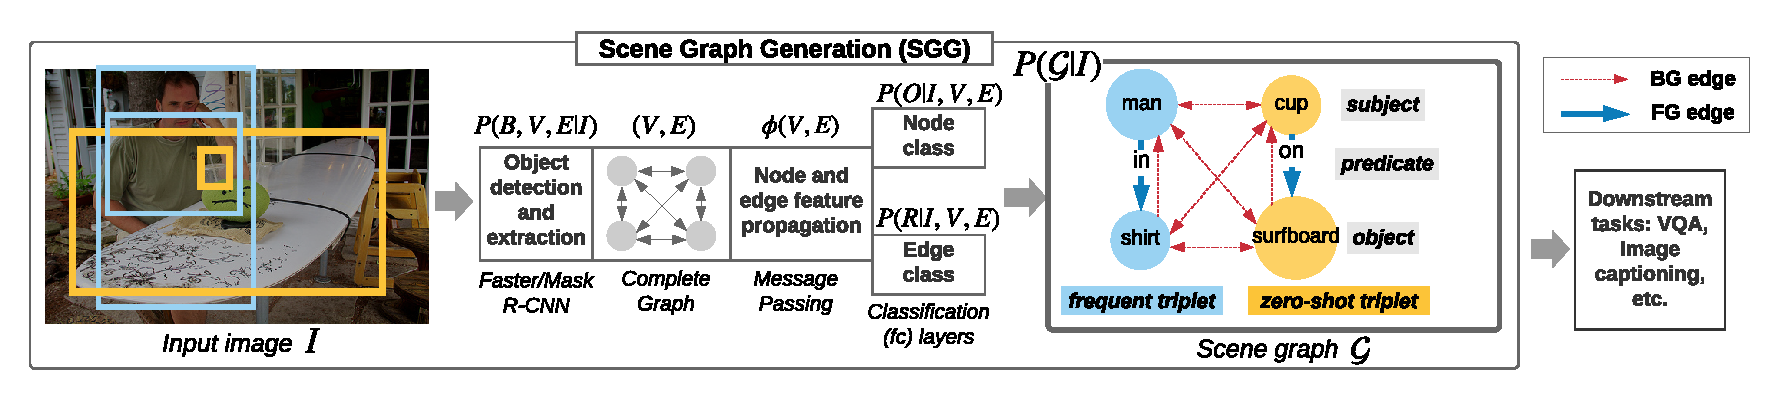
\includegraphics[width=0.99\textwidth,align=c,trim={0 0.2cm 0 0.2cm},clip]{2020_bmvc/figs/cup_on_surfboard_overview1.pdf} \\
% 		\end{tabular}
% 	\end{scriptsize}
% 	\vspace{-5pt}
% 	\caption{\small Typical scene graph generation pipeline used in high-level visual reasoning tasks (figure from~\citep{knyazev2020graph}). Foreground (FG) edges denote annotated relations, while background (BG) ones denote the absence of relations as deemed by the annotator or annotation system.} %In many downstream tasks, such as VQA, the result directly depends on the accuracy of predicted scene graphs.}
% 	\label{fig:overview_sg}
% \end{figure}

\begin{figure}[thbp]
	\centering
	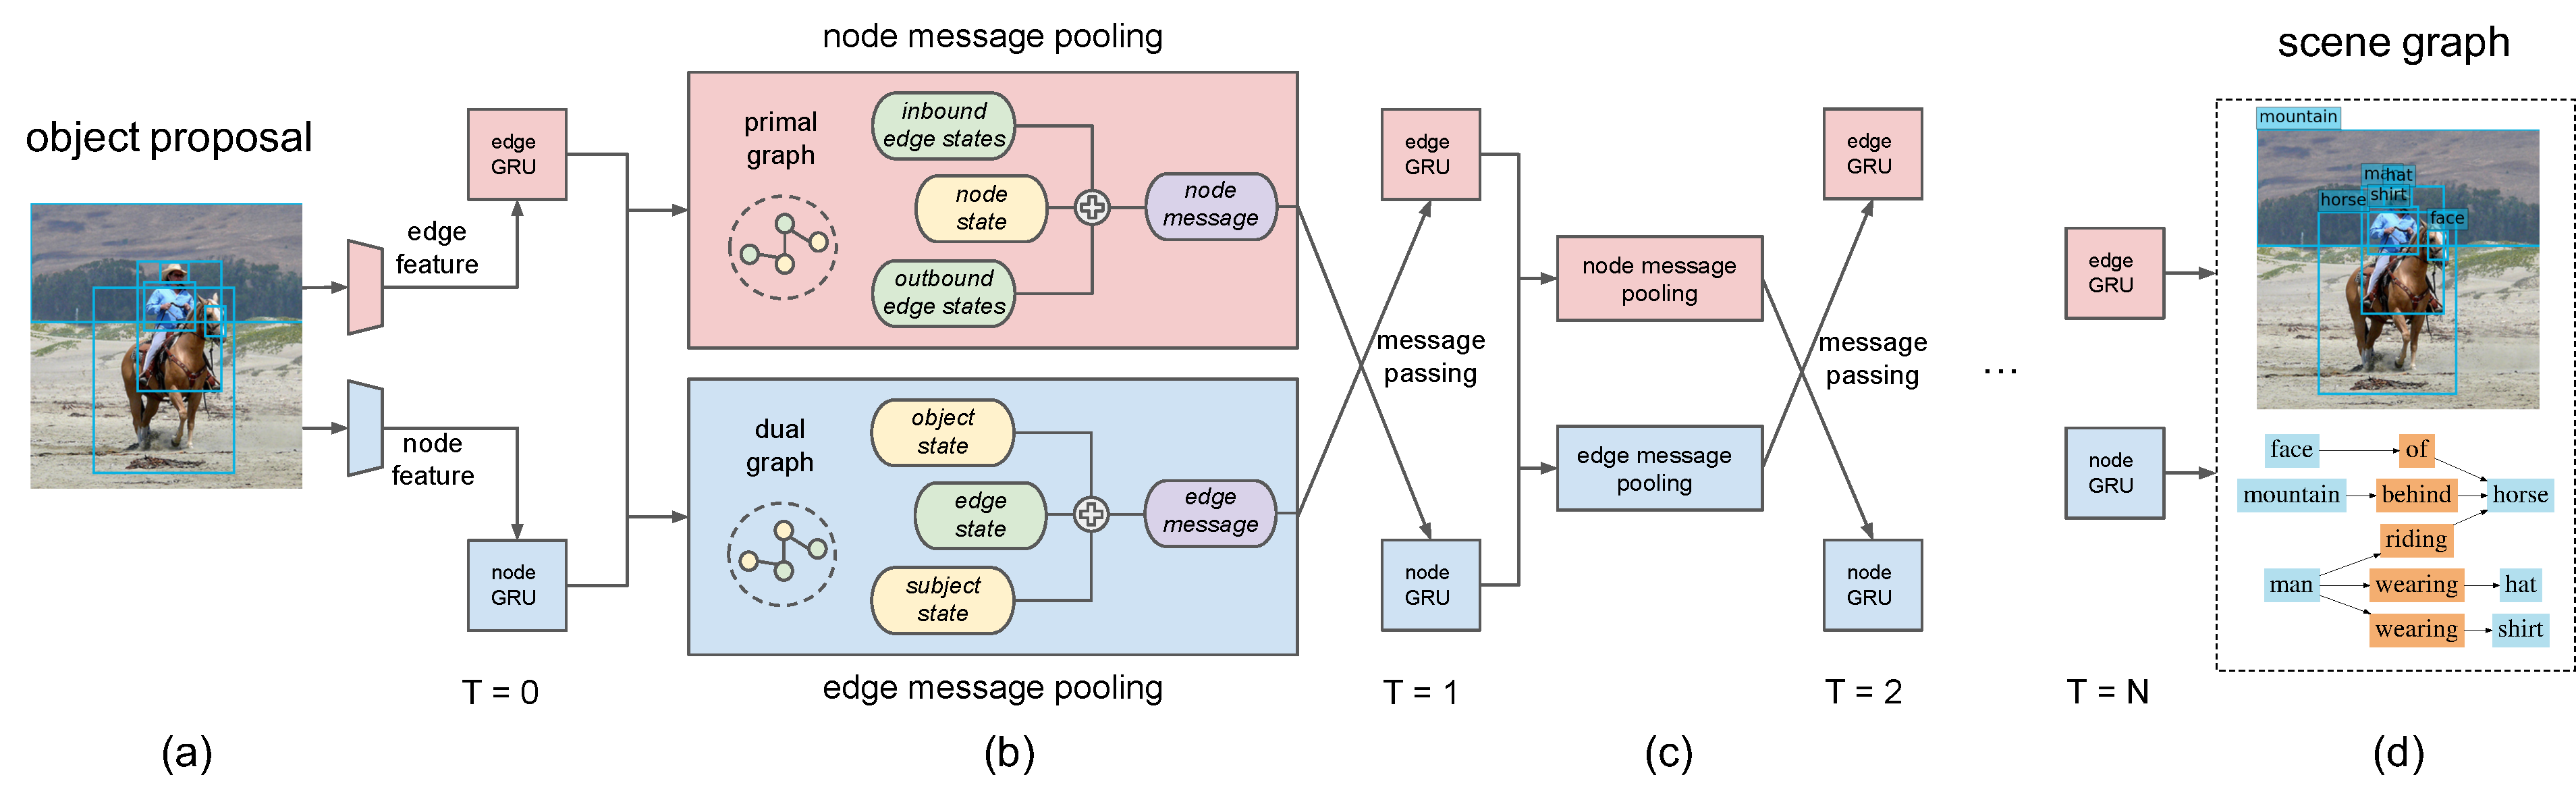
\includegraphics[width=0.99\textwidth,align=c,trim={0 2.1cm 0cm 0.2cm},clip]{figs/stanford_network.pdf}
	%\vspace{-5pt}
	\caption{\small A scene graph generation model from~\citep{xu2017scene} used in high-level visual reasoning tasks. This and other SGG models~\citep{yang2018graph} are often based on message passing networks that resemble graph neural networks~\citep{gilmer2017neural,battaglia2018relational}.}
	\label{fig:overview_sg}
\end{figure}

%In scene graph generation} (SGG) the task is to predict a scene graph (SG) given an input image. %The inferred SG can be used directly for downstream tasks such as VQA~\citep{zhang2019empirical,NSM2019}, image captioning~\citep{yang2019auto, gu2019unpaired} or retrieval~\citep{johnson2015image,belilovsky2017joint,tang2020unbiased}.
%A model which performs well on SGG should demonstrate the ability to ground visual concepts to images and generalize to compositions of objects and predicates in new contexts.
% \paragraph{Overview of Scene Graph Generation}
% 	\label{sec:baseline}
Extracting a scene graph $\cal G$ from an image $I$ is a standard high-level visual reasoning task and is called scene graph generation (SGG)~\citep{xu2017scene}. In general, SGG models first extract a complete graph from an image, where nodes correspond to detected objects~\citep{zellers2018neural,yang2018graph}. Then several message passing rounds update node and edge features. The goal of the SGG model is to predict a sparse scene graph $\cal G$ given the dense graph of node and edge features (\fig{\ref{fig:overview_sg}}).
Typically, many different $\cal G$ can be valid for a single image $I$, so obtaining $\cal G$ resembles a generative process. However, in practice there is typically only one ground-truth $\cal G$ annotated for each image and the SGG models are typically deterministic, so the task is rather ``scene graph prediction''. Nevertheless, we will use the term SGG to be consistent with the scene graph literature.


\subsection{Compositional generalization\label{sec:bg_comp_gen}}

In real world images, some compositions, \eg~$\langle$cup, on, table$\rangle$ or $\langle$person, on, surfboard$\rangle$, appear more frequently than other unusual ones, \eg~$\langle$cup, on, \textit{surfboard}$\rangle$, $\langle$cup, \textit{under}, table$\rangle$ or $\langle$\textit{dog}, on, surfboard$\rangle$. %, which creates a strong frequency bias. 
Such a difference in frequencies -- the \textit{frequency bias} -- is often present in commonly-used visual relationship datasets, such as Visual Genome~\citep{krishna2017visual}.
% (\fig{\ref{fig:motivation_gan}}). 
The frequency bias is purely statistical and poorly reflects the physical plausibility of object interactions. For example, according to the statistics of Visual Genome the probability of $\langle$cup, on, {surfboard}$\rangle$ is exactly zero because such a composition has never occurred. However, from the physical point of view (in the real world), such a composition would have a greater than zero probability. In fact, $\langle$cup, on, {surfboard}$\rangle$ appears in the test set of Visual Genome.
%of  and are often called the frequency bias.
The ability of models to recognize such novel (\textit{zero-shot} or ZS) and rare (\textit{few-shot} or FS) compositions accurately, despite the frequency bias, is called \textit{\cg} (\cgshort). 
Compositional generalization has been widely studied in the language~\citep{atzmon2016learning, keysers2019measuring, lake2019compositional} and reinforcement learning domains~\citep{jiang2019language,cogswell2019emergence,kipf2019compile}, as well as multi-domain tasks~\citep{johnson2017clevr,bahdanau2018systematic,bahdanau2019closure,agrawal2017c,agrawal2018don}.
In the visual domain, compositional reasoning has been addressed in the scene graph generation (SGG) task and image classification from attributes~\citep{lampert2013attribute,demirel2017attributes2classname,naeem2021learning} (\fig{\ref{fig:zeroshots}}).

\begin{figure}[thbp]
	\centering
	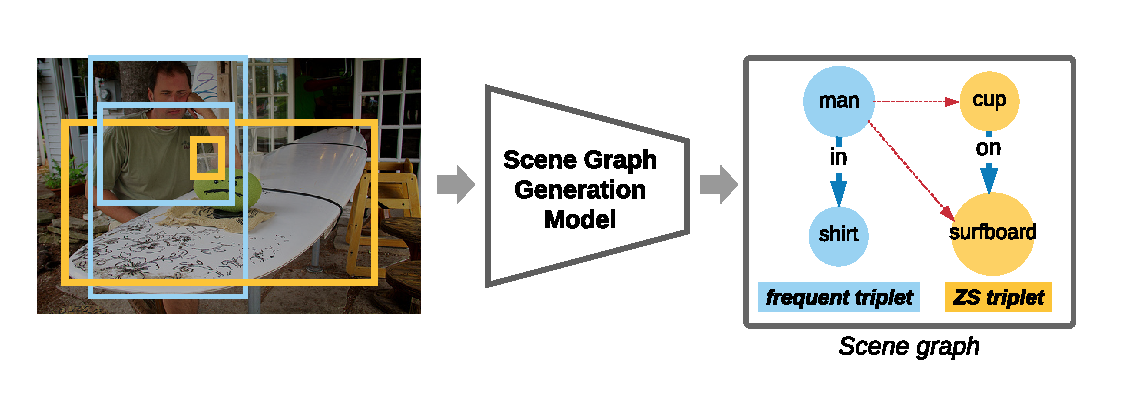
\includegraphics[width=0.99\textwidth,align=c,trim={0 0cm 0cm 0cm},clip]{figs/zeroshots.pdf}
	\vspace{-15pt}
	\caption{\small An example of a ground truth scene graph with a zero-shot composition (ZS triplet) that must be predicted by an SGG model for an input image. The figure is adapted from~\citep{knyazev2020graph}. Dashed red arrows denote the relationships that have not been annotated by a human.}
	\label{fig:zeroshots}
\end{figure}

%So, unless the models have a strong inductive prior , they will tend to predict `person' rather than `dog' on a surfboard. 
While compositional reasoning about concepts is easy for humans, for machines this task has remained extremely challenging. 
The reasons for the challenging nature of \cgshort are not well understood.
The challenge may relate to the fact that learning-based models tend to capture spurious statistical correlations and biases of datasets during training~\citep{arjovsky2019invariant,niu2020counterfactual,tang2020unbiased}. 
%The frequency bias of visual relationship datasets is particularly pronounced making it hard for the models to recognize relationships without relying on the bias.
The frequency bias of visual relationship datasets is particular pronounced, so for the learning-based models it is hard to not rely on this bias.
%The presence of the strong frequency bias in data and the tendency of models to rely on this bias make the \cgshort problem extremely challenging.
The \cgshort challenge has been largely overlooked, since the test sets often have the same frequency bias and the evaluation metrics do not penalize models for blindly relying on the bias. However, when the evaluation is explicitly focused on \cgshort, the models have been found to fail remarkably~\citep{atzmon2016learning, lu2016visual, tang2020unbiased, knyazev2020graph}.

In the SGG task, recall-based metrics are typically used for evaluation. So, on frequent compositions these metrics can reach $\sim$41\%, while on zero-shot compositions the state-of-the-art result is only 4.5\% -- a nearly 10 fold drop in performance~\citep{tang2020unbiased}.
Previous SGG works often assume \cgshort is similar to few-shot predicate generalization and so attempt to improve mean (or predicate-normalized) recall metrics that are not directly related to \cgshort~\citep{chen2019knowledge, dornadula2019visual,tang2019learning,zhang2019graphical,tang2020unbiased,chen2019scene,zareian2020bridging,yan2020pcpl}.  
Predicate imbalance can be treated by simple resampling-based methods, while \cgshort is more challenging~\citep{tang2020unbiased}. Therefore, \cgshort rather than predicate imbalance has to be a focus of visual reasoning tasks.


\subsection{Methods to improve compositional generalization\label{sec:bg_methods}}

The methods to improve visual \cg (\cgshort) can be grouped into two categories. These are: methods that explicitly impose some compositional inductive prior on the models, and those where \cgshort comes, or can potentially come, as a side-effect. The side-effect can be, for example, a result of a regularization method applied to neural networks.\looseness-1

\paragraph{Explicit Compositionality.}
Methods to introduce explicit compositionality can be grouped into high-level and lower-level reasoning tasks. The works on other forms of generalization related to high-level \cg are also discussed.

\begin{itemize}[leftmargin=5mm]
    \item \textbf{High-level visual reasoning}: High-level visual \cgshort was first evaluated in~\citep{lu2016visual} on the VRD dataset using a joint vision-language model.
    Several follow-up works attempted to improve upon it: by learning a translation operator in the embedding space~\citep{zhang2017visual}, clustering in a weakly-supervised fashion~\citep{peyre2017weakly}, using conditional random fields~\citep{cong2018scene} or optimizing a cycle-consistency loss to learn object-agnostic features~\citep{yang2018shuffle}. Augmentation using generative models to synthesize more examples of rare compositions is another promising approach~\citep{wang2019generating}, because we can generate many instances of rare compositions mitigating the frequency bias. 
    But, in \citep{wang2019generating} this approach was only evaluated on a simple predicate classification task.
    %In our work, we also consider subject/object classification to enable the classification of the whole triplets, making the ``image to scene graph'' pipeline complete. 
    Most recently,~\citet{tang2020unbiased} proposed to mitigate the bias by inferring causal rather than correlated relationships and, consequently, showed strong performance on zero-shot visual compositions. In a subsequent work, \citet{suhail2021energy} improved the SGG loss function \eqref{eq:scene_graph_prob_simple} to reduce the bias and better handle \cgshort.
    %In the visual domain, compositionality has been introduced in the form of translation operators~\citep{zhang2017visual}, decoupling object and predicate features~\citep{yang2018shuffle} and constructing causal graphs~\citep{tang2020unbiased}.
    In the VQA task, compositionality has been improved by predefining neural modules~\citep{andreas2016neural} and their more flexible end-to-end extensions \citep{hu2017learning,johnson2017inferring}.
    However, since the VQA task often relies on accurately extracting scene graphs, the methods that impose a compositional prior on scene graph prediction improve \cgshort in VQA~\citep{yi2018neural,mascharka2018transparency,shi2019explainable}.
    
    \item %Explicit compositionality has been introduced in lower-level reasoning tasks such as image and attribute classification. 
    \textbf{Lower-level visual reasoning}: The area of low-level visual reasoning is less organized and there is no standard evaluation benchmark. So different works have focused on different aspects of compositionality at the level of simple objects, object parts and attributes. In particular, to improve compositionality of simple objects, a mask-based loss term was added to image classification networks in~\citep{stone2017teaching}. However, this loss requires expensive pixel-wise mask annotations for training images. 
    %However, the loss was shown to improve compositionality.
    In another work~\citep{sylvain2019locality}, to improve generalization to unseen object categories, a more local representation using self-supervised objectives based on Deep InfoMax~\citep{hjelm2018learning} was learned. 
    %To recognize novel object categories, compositional understanding at the level of object parts and attributes is essential.
    Zero-shot object classification was also studied in~\citep{tokmakov2019learning}. The model in \citep{tokmakov2019learning} is based on decomposing the image representation into a set of attribute representations in the visual space. However, the model does not require to annotate attributes for novel classes to predict their labels.
    Generalization to zero-shot objects and object-attribute compositions may be approached by learning an image extraction \cnn together with a \gnn that learns a knowledge graph from existing object categories and their attributes~\citep{naeem2021learning}. 
    Another approach to this task is based on a prototypical model that learns object representations disentangled from attribute representations to enable strong generalization to unseen compositions of objects and attributes~\citep{ruis2021independent}. To further progress in the lower-level \cgshort, more standardized benchmarks are needed. Integration of the lower-level and higher-level \cgshort methods and evaluation protocols can also enable faster progress towards better generalization in visual reasoning.
    
    \item \textbf{Other tasks}: Several general methods exist that can be potentially useful for \cgshort. One such method is unsupervised domain adaptation (UDA) by backpropagation~\citep{ganin2015unsupervised} closely connected to domain-adversarial neural networks\citep{ajakan2014domain,JMLR:v17:15-239}. UDA achieved strong results by learning features invariant to the domain. Such a model allows to recognize objects in novel domains and contexts.
    Another general method is meta-learning~\citep{hospedales2020meta} that typically targets few-shot generalization in classification tasks. 
    The idea of commonly-used meta-learning methods, such as MAML~\citep{finn2017model}, is to take the original training dataset and split it into a sequence of training and validation subsets (episodes). The critical part is to make the validation set largely composed of few-shot data. This way, the meta-learning algorithm aims to update the parameters of a model on the validation loss thereby improving it by learning to generalize to a few examples. In compositional language reasoning, such a meta-learning based objective was proposed in~\citep{lake2019compositional}, where the validation set is largely composed of zero and few shot compositions. This method yielded improvement \cgshort on language tasks, and potentially, can be applied to visual tasks.
\end{itemize}


\paragraph{Implicit Compositionality via Object-centric Learning.}

Unsupervised learning has recently received more attention in different visual tasks~\citep{radford2015unsupervised,hjelm2018learning,chen2020simple,verma2021towards}, and is potentially useful for \cgshort as well.
In particular, one of the reasons for poor \cgshort of models might be the biased annotations in the datasets on which models are trained. Therefore, a logical way to mitigate such bias is to rely less on the annotations. In an extreme case, we can train a model without any labels, in a purely unsupervised fashion.
In the context of compositional visual reasoning, a growing body of unsupervised learning works focus on object-centric learning~\citep{greff2020binding}, usually by employing an encoder-decoder model~\citep{engelcke2019genesis,burgess2019monet,greff2019multi,locatello2020object}.
Object-centric learning methods generally decompose an image representation into a set of object representations without accessing the labels of the objects. Some methods also allow to disentangle physical attributes of objects, such as color, shape and material~\citep{greff2019multi}. The decomposition of an image into objects is typically done by iteratively running encoder-decoder inference until the image is fully reconstructed~\citep{greff2019multi}. 
%The method in~\citep{greff2019multi} allows to not only separate objects from each other, but also to disentangle objects from their physical attributes. 
Due to its iterative nature, the inference procedure is computationally inefficient.
Another method, slot attention~\citep{locatello2020object}, is more efficient, since it only requires a single encoder iteration to extract all object representations. Yet, it is unclear if this model disentangles object attributes as in~\citep{greff2019multi}. Slot attention is reminiscent to the k-means clustering method. Unlike k-means, slot attention is fully-differentiable and employs self-attention~\citep{vaswani2017attention} with the softmax function to enforce more sparse representation. Object-centric learning methods are typically evaluated using pixel-wise segmentation metrics similar to earlier unsupervised semantic segmentation works~\citep{arbelaez2010contour}.
In addition, in \citep{locatello2020object,greff2019multi} the evaluation includes how well the representation encodes visual object properties.
Overall, object-centric learning is a promising direction for \cgshort as it enables an unbiased (w.r.t. human annotations) decomposition of images into entities that often have a semantic meaning. Such unbiased decomposition recently allowed object-centric learning methods to improve results on several out-of-distribution generalization tasks~\citep{dittadi2021generalization}.\looseness-1

\paragraph{Implicit Compositionality via Regularized Training.}

Regularization methods are often aimed at reducing overfitting and improving different generalization abilities. An open question remains whether or not these methods can also improve \cgshort.
% Among the regularization methods to reduce overfitting and improve overall generalization, 
In the following, the methods that can be more directly leveraged for compositional generalization are considered.

Let us consider the feature activations after some layer $l$: $\X^{(l)} \in \R^{N \times d_l}$, where 
$N$ is the number of data points (in a batch) and
%$n \in [1, N]$ is an index of a sample in the batch of $N$ sample and 
$d_l$ is dimensionality\footnote{$\X^{(l)}$ can be outputs of a fully-connected, convolutional, graph layer, etc. In the case of 2D or 3D dimensions in $\X^{(l)}$, such as after convolutions, it can be flattened to a 1D tensor.\looseness-1}. 
To index the $i$-th individual feature (scalar) of the $n$-th sample, the notation $\X_{n,i}$ will be used.
In the visual domain, when a \cnn is used to extract $\X$, these activations tend to be highly-correlated due to the regularities in the input data and co-adaptation of weights to capture those regularities~\citep{hinton2012improving}, \ie the probability $p(\X_{n,i} | \X_{n,j})$ tends to be high. For example, if the $i$-th feature is activated when the input image contains `surfboard', then the $j$-th feature associated with the entity `person' is likely to be activated regardless if the image actually contains the `person' or another object such as `dog'. On the one hand, relying on co-adaptation allows neural networks to fit data more easily. %similarly as relying on (spurious) context in %high-level visual reasoning. 
On the other hand, heavy reliance on co-adaptation can hurt generalization, so some regularization strategies are needed to mitigate that.\looseness-1

Many regularization strategies to alleviate overfitting have been proposed. One common strategy is Dropout~\citep{hinton2012improving}: $\text{dropout}(\X, r)$. Dropout stochastically sets to zero the values of $\X$ with probability $r$ during training. \citet{ghiasi2018dropblock} generalized this method to convolutions by setting to zero locally connected activations rather than arbitrary ones.
In contrast, \citet{cogswell2015reducing} proposed a covariance loss penalty to explicitly reduce correlation of features.
Adding the loss penalty to the task objective helped the networks to obtain better generalization properties compared to using Dropout. 
However, due to the expensive procedure of computing covariance, this approach does not scale well to high-dimensional features typically present in visual tasks. 
This limitation was addressed by introducing a locally connected decorrelation penalty specific for convolutional features~\citep{rodriguez2016regularizing}.
Instead of adding a loss penalty~\citep{cogswell2015reducing,rodriguez2016regularizing}, enforcing orthogonality on weights in \cnns during initialization may help to better regularize the model and, subsequently, achieve better generalization results~\citep{bansal2018can,wang2020orthogonal}. However, it is important to maintain the orthogonality regularization during the whole training procedure, because the weights tend to diverge to a poor solution otherwise~\citep{wang2020orthogonal}. Alternatively, generalization can also be improved using decorrelated batch normalization (BN)~\citep{huang2018decorrelated}, which can also be viewed as a form of regularization. While decorrelated BN improves generalization compared to original BN~\citep{ioffe2015batch}, it remains unclear if decorrelated BN is better for generalization than other regularization strategies, such as orthogonal regularization.\looseness-1

The discussed regularization methods mainly improve generalization results in a more classic machine learning sense, such as generalization to the in-distribution test images.
%, they only address the linear independence of features. Nonlinear correlations and, hence redundancy, can be well present in networks. Moreover,
However, except for a few synthetic experiments in~\citep{cogswell2015reducing}, the effect of these methods on out-of-distribution and, especially, compositional generalization has not been systematically evaluated. Meanwhile, these regularization techniques, in particular the orthogonal one, can facilitate learning a representation where entities are more (linearly) independent, and hence disentangled, from each other. This might directly improve \cgshort, which needs to be empirically confirmed.
